\documentclass[12pt,a4paper]{report}
\usepackage[utf8]{inputenc}
\usepackage[top=2cm,bottom=2cm,right=2cm,left=2cm]{geometry}
\usepackage{amsmath,amsfonts,amssymb,mathrsfs,tikz,fancybox}
\pagestyle{empty}
\usetikzlibrary{arrows,shapes}
\def\sh{
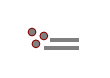
\begin{tikzpicture}[scale=0.05,rotate=-90]
\draw[line width=.3pt,fill=gray,draw=red!50!black](0,0)circle(1cm);
\draw[line width=.3pt,fill=gray,draw=red!50!black](3,1)circle(1cm);
\draw[line width=.3pt,fill=gray,draw=red!50!black](1,3)circle(1cm);
\draw [line width=1.5pt,gray](2,4.5)--(2,12);
\draw [line width=1.5pt,gray](4,3)--(4,12);
\end{tikzpicture}
}
\begin{document}
\begin{tikzpicture}[remember picture,overlay]
\foreach \i in {1,...,44}{
\path ([shift={(45:1)}]current page.south west)|-
node[sloped,pos=\i/90]{\sh}
([shift={(225:1)}]current page.north east);
\path ([shift={(135:1)}]current page.south east)|-
node[sloped,pos=\i/90]{\sh}
([shift={(-45:1)}]current page.north west);}
\foreach \i in {1,...,29}{
\path ([shift={(45:1)}]current page.south west)--
node[sloped,pos=\i/30]{\sh}
([shift={(135:1)}]current page.south east);
\path ([shift={(-45:1)}]current page.north west)--
node[sloped,pos=\i/30]{\sh}
([shift={(225:1)}]current page.north east);
}
\foreach \m/\j in {-45/north west,225/north east,45/south west,135/south east}{
\draw [line width=1.5pt,red!50!black,fill=gray]([shift={(\m:1)}]current page.\j)circle(2mm);
}
\end{tikzpicture}
{\centering\sl\bfseries
République Algérienne démocratique et Populaire\\
Ministère de l'enseignement supérieur et de la recherche scientifique
\vskip6mm\large
UNIVERSITE Dr.TAHAR MOULAY SAIDA\\[3mm]
\rm\bf\normalsize
FACULTE : TECHNOLOGIE\\[3mm]
DEPARTEMENT : INFORMATIQUE
\vskip6mm
\includegraphics[width=4cm,height=1.5cm]{logo}
\vskip5mm\sl
\underline{\bf\Large MEMOIRE DE MASTER}
\vskip1cm\rm\bf
OPTION:
\vskip1.5cm
\begin{center}
\underline{\slshape\bfseries Thème}
\vskip3mm
\ovalbox{\parbox[c][3cm][c]{\textwidth}{\centering
\bfseries\huge
LE TITRE DU MEMOIRE
}}
\end{center}
\vfill
\begin{minipage}[t]{8cm}
\underline{\bf Présenté par:}\\[3mm]\bf
Nom et prénom
\end{minipage}
\hfill
\begin{minipage}[t]{5cm}
\underline{\bf Enquadré par:}\\[3mm]\bf
\hfill Nom \& Prénoms
\end{minipage}
\vfill
\centering\bf
Promotion: mois \& année
\end{document}